\begin{figure}[H] 
  \begin{subfigure}[b]{0.5\linewidth}
    \centering
    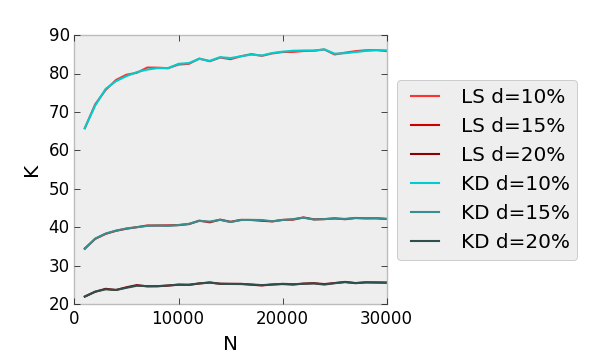
\includegraphics[width=0.9\linewidth]{Pictures/unif_kd_ls_k} 
    %\caption{$N=10$} 
    \label{fig:unif_kd_ls_k} 
    \vspace{4ex}
  \end{subfigure}%% 
  \begin{subfigure}[b]{0.5\linewidth}
    \centering
    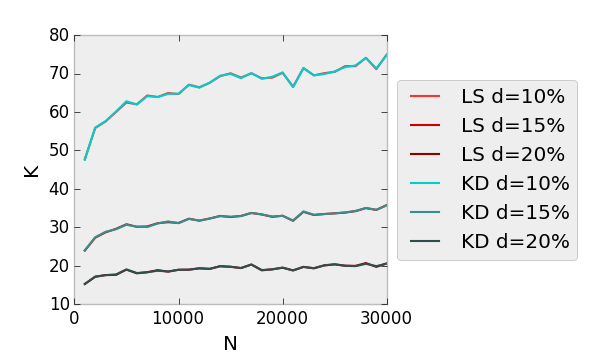
\includegraphics[width=0.9\linewidth]{Pictures/clus_kd_ls_k} 
    %\caption{$N=20$} 
    \label{fig:clus_kd_ls_k} 
    \vspace{4ex}
  \end{subfigure}
  \caption[Number $K$ of points selected for Line Sweep and $k$-d Tree range search]{Number $K$ of points selected for both proximity graph algorithms on uniform inputs(left) and clustered inputs(right).}
  \label{fig:kd_ls_k} 
\end{figure}

